% !TEX TS-program = pdflatex
% !TEX encoding = UTF-8 Unicode

%************************************************
\chapter{Sistema di diffusione}
\label{chp:Sistema di diffusione}
%************************************************

\epigraph{Come un rosone nel cuore di un tempio immenso}{\textit{Antonin Artaud}}

La diffusione sonora di Vitres de Son è basata sull'utilizzo di 9 dei 22 altoparlanti (più il sub-woofer) presenti nella cupola sonora "Il suono di Piero" costruita nel all'interno dell'Aula I del III piano del conservatorio Santa Cecilia. \begin{figure}[!htbp]
\begin{center}
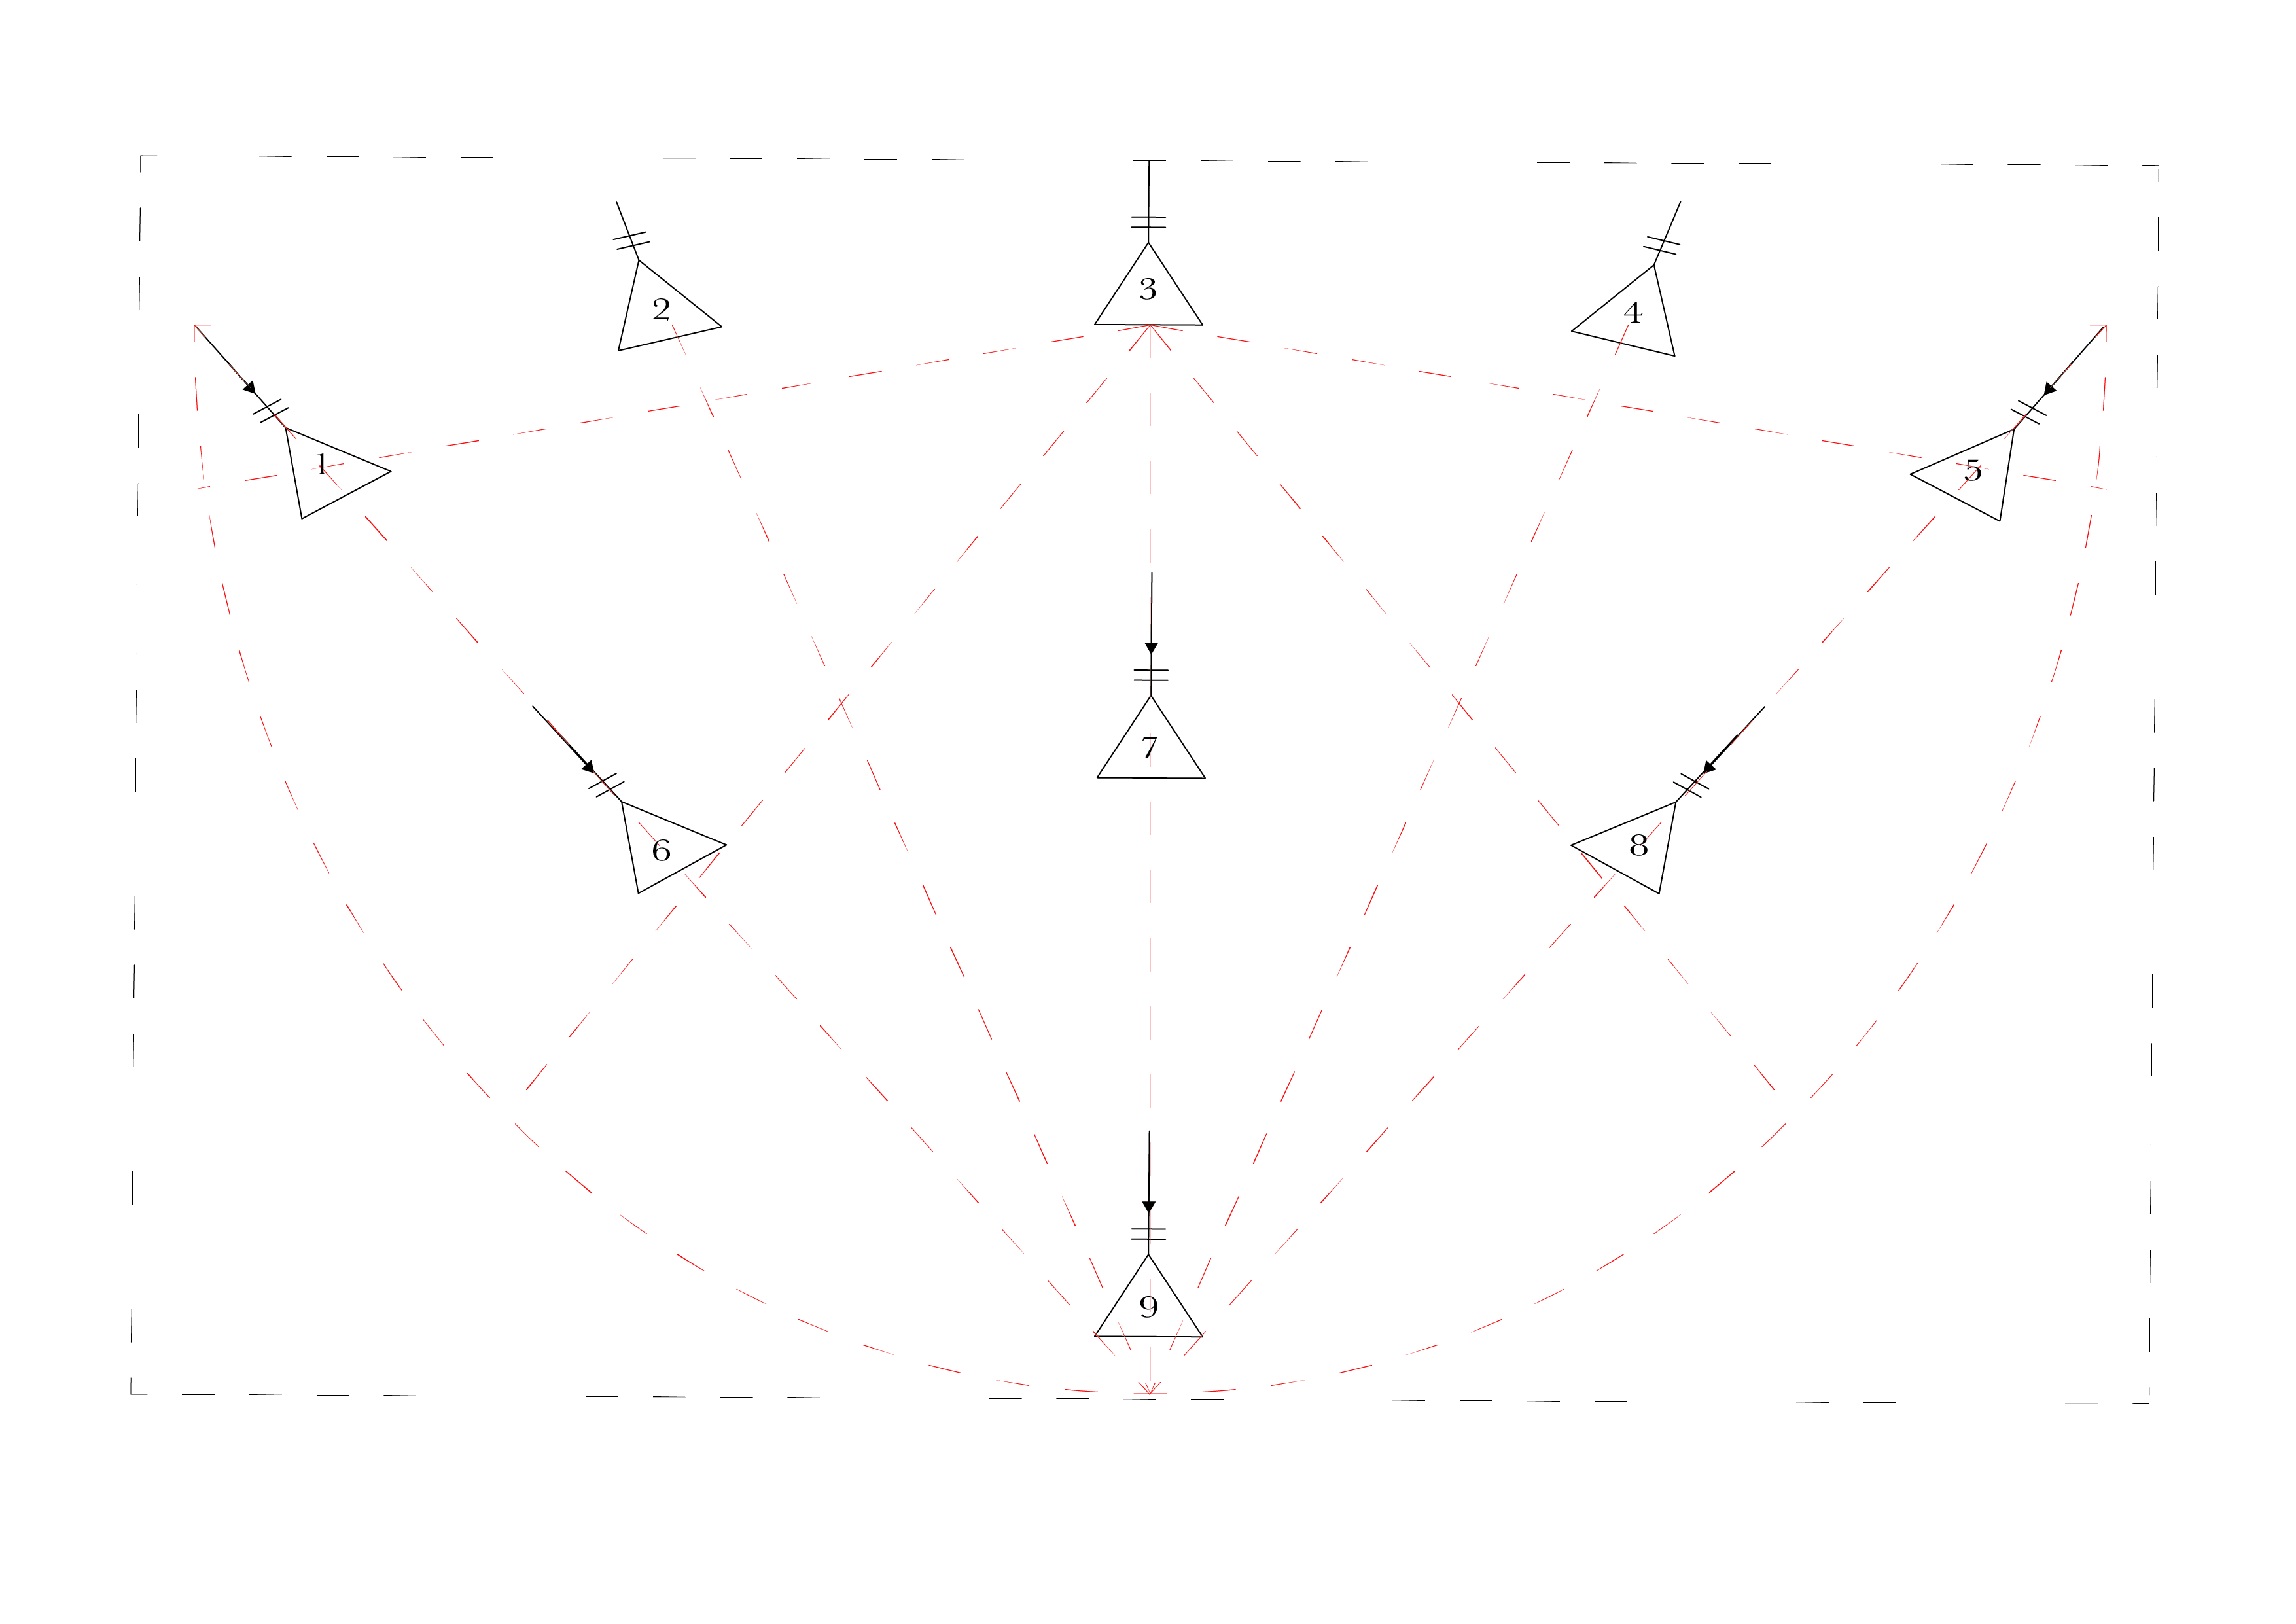
\includegraphics[width=1\textwidth]{legenda02.png}
\caption{Diffusione a \textit{A Rosone} di Vitres de Son}
\label{default}
\end{center}
\end{figure}Sfruttare solo una parte della cupola è legato alle mie esigenze composizione, sia a livello di figura nella quale far adagiare l'esecutore che lo Sp.I.R.E.. Come rappresentato nella figura qui sopra, notiamo che i diffusori più esterni sono i vertici di un triangolo inscritto in un arco: significante dell'immagine del rosone. Il suono confluisce al centro e la microfonazione ci dà la possibilità di apprezzarlo nei suoi spostamenti. Sottolineo, inoltre, che la spazializzazione è data esclusivamente dall'amplificazione trasparente.
Per la costruzione del sistema di diffusione ho utilizzo gli scritti introduttivi che sono allegati a molte partiture di Luigi Nono e Karlheinz Stockhausen (che verranno svelate in seguito). Il compositore non è più slegato da una realtà percettiva e teatrale del produzione sonora, ma diventa artefice della disposizione degli altoparlanti e del pubblico all'interno dell'ambiente d'ascolto.
Vediamo nel dettaglio il sistema di ripresa e la diffusione audio che da partitura diventano parte integrante della composizione.

\section{Sistema di ripresa}
La diffusione audio avverrà tramite l'utilizzo di un sistema di ripresa omnidirezionale che renderà possibile la diffusione omogenea del materiale acustico ed elettronico prodotto da Sp.i.r.e..
\begin{figure}[!htbp]
\begin{center}
\includegraphics[width=.99\textwidth]{ripresa.jpg}
\caption{Ripresa microfonica dello Sp.I.R.E.}
\label{default}
\end{center}
\end{figure}
Di seguito, i materiali tecnici da utilizzare per la riproduzione dell'opera:
\begin{itemize}
	\item{Scheda Audio 8in 9out}
	\item{Mixer Yamaha DM1000}
	\item{4 piezoelettrici}
	\item{2 microfoni dpa omnidirezionali}
	\item{2 microfoni Cardioide Neumann}
	\item{Cablaggio}
	\item{1 Amplificatore di potenza da 4 canali a 4 Ohm}
	\item{Computer\\}
\end{itemize}

\section{Diffusione} 

Per schematizzare e disegnare la diffusione audio, ho utilizzato come esempio gli scritti introduttivi e le legende di due partiture contemporanee. Specificatamente: \textit{Mantra} di Karlheinz Stockhausen e \textit{Prometeo, Tragedia dell'ascolto} di Luigi Nono. Nella partitura di Stockhausen

\begin{figure}[htbp]
\begin{center}
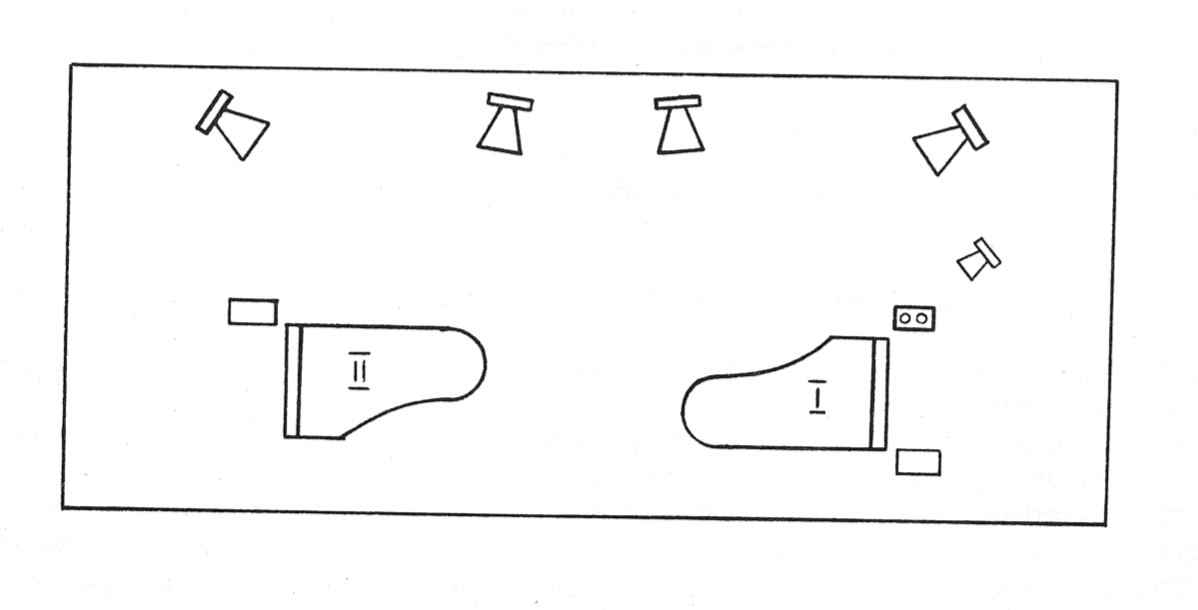
\includegraphics[width=.99\textwidth]{Mantra.jpg}
\caption{Particolare della Legenda di \textit{Mantra}}
\label{default}
\end{center}
\end{figure}

vediamo come il compositore esplica lucidamente il rapporto che c'è tra diffusione ed elaborazione del segnale, in un solo schema racchiude sia la diffusione che l'elaborazione.
Nono, nel Prometeo, aggiunge agli schemi algoritmici e di diffusione, anche la disposizione del pubblico in sala. Questa è un passo importante per la storia della musica elettroacustica, perché alla modalità d'ascolto si aggiunge un fattore importante per la stesura di un lavoro compositivo: la regia. Nono era sempre attento al rapporto fra diffusione del suono e disposizione dell'ascoltatore.
Prendendo ad esempio i maestri, ho lavorato su un'irradiazione tale da poter favorire un spostamento del suono a livello spaziale. La tipologia di microfonazione e la disposizione dei diffusori, permette:

\begin{figure}[htbp]
\begin{center}
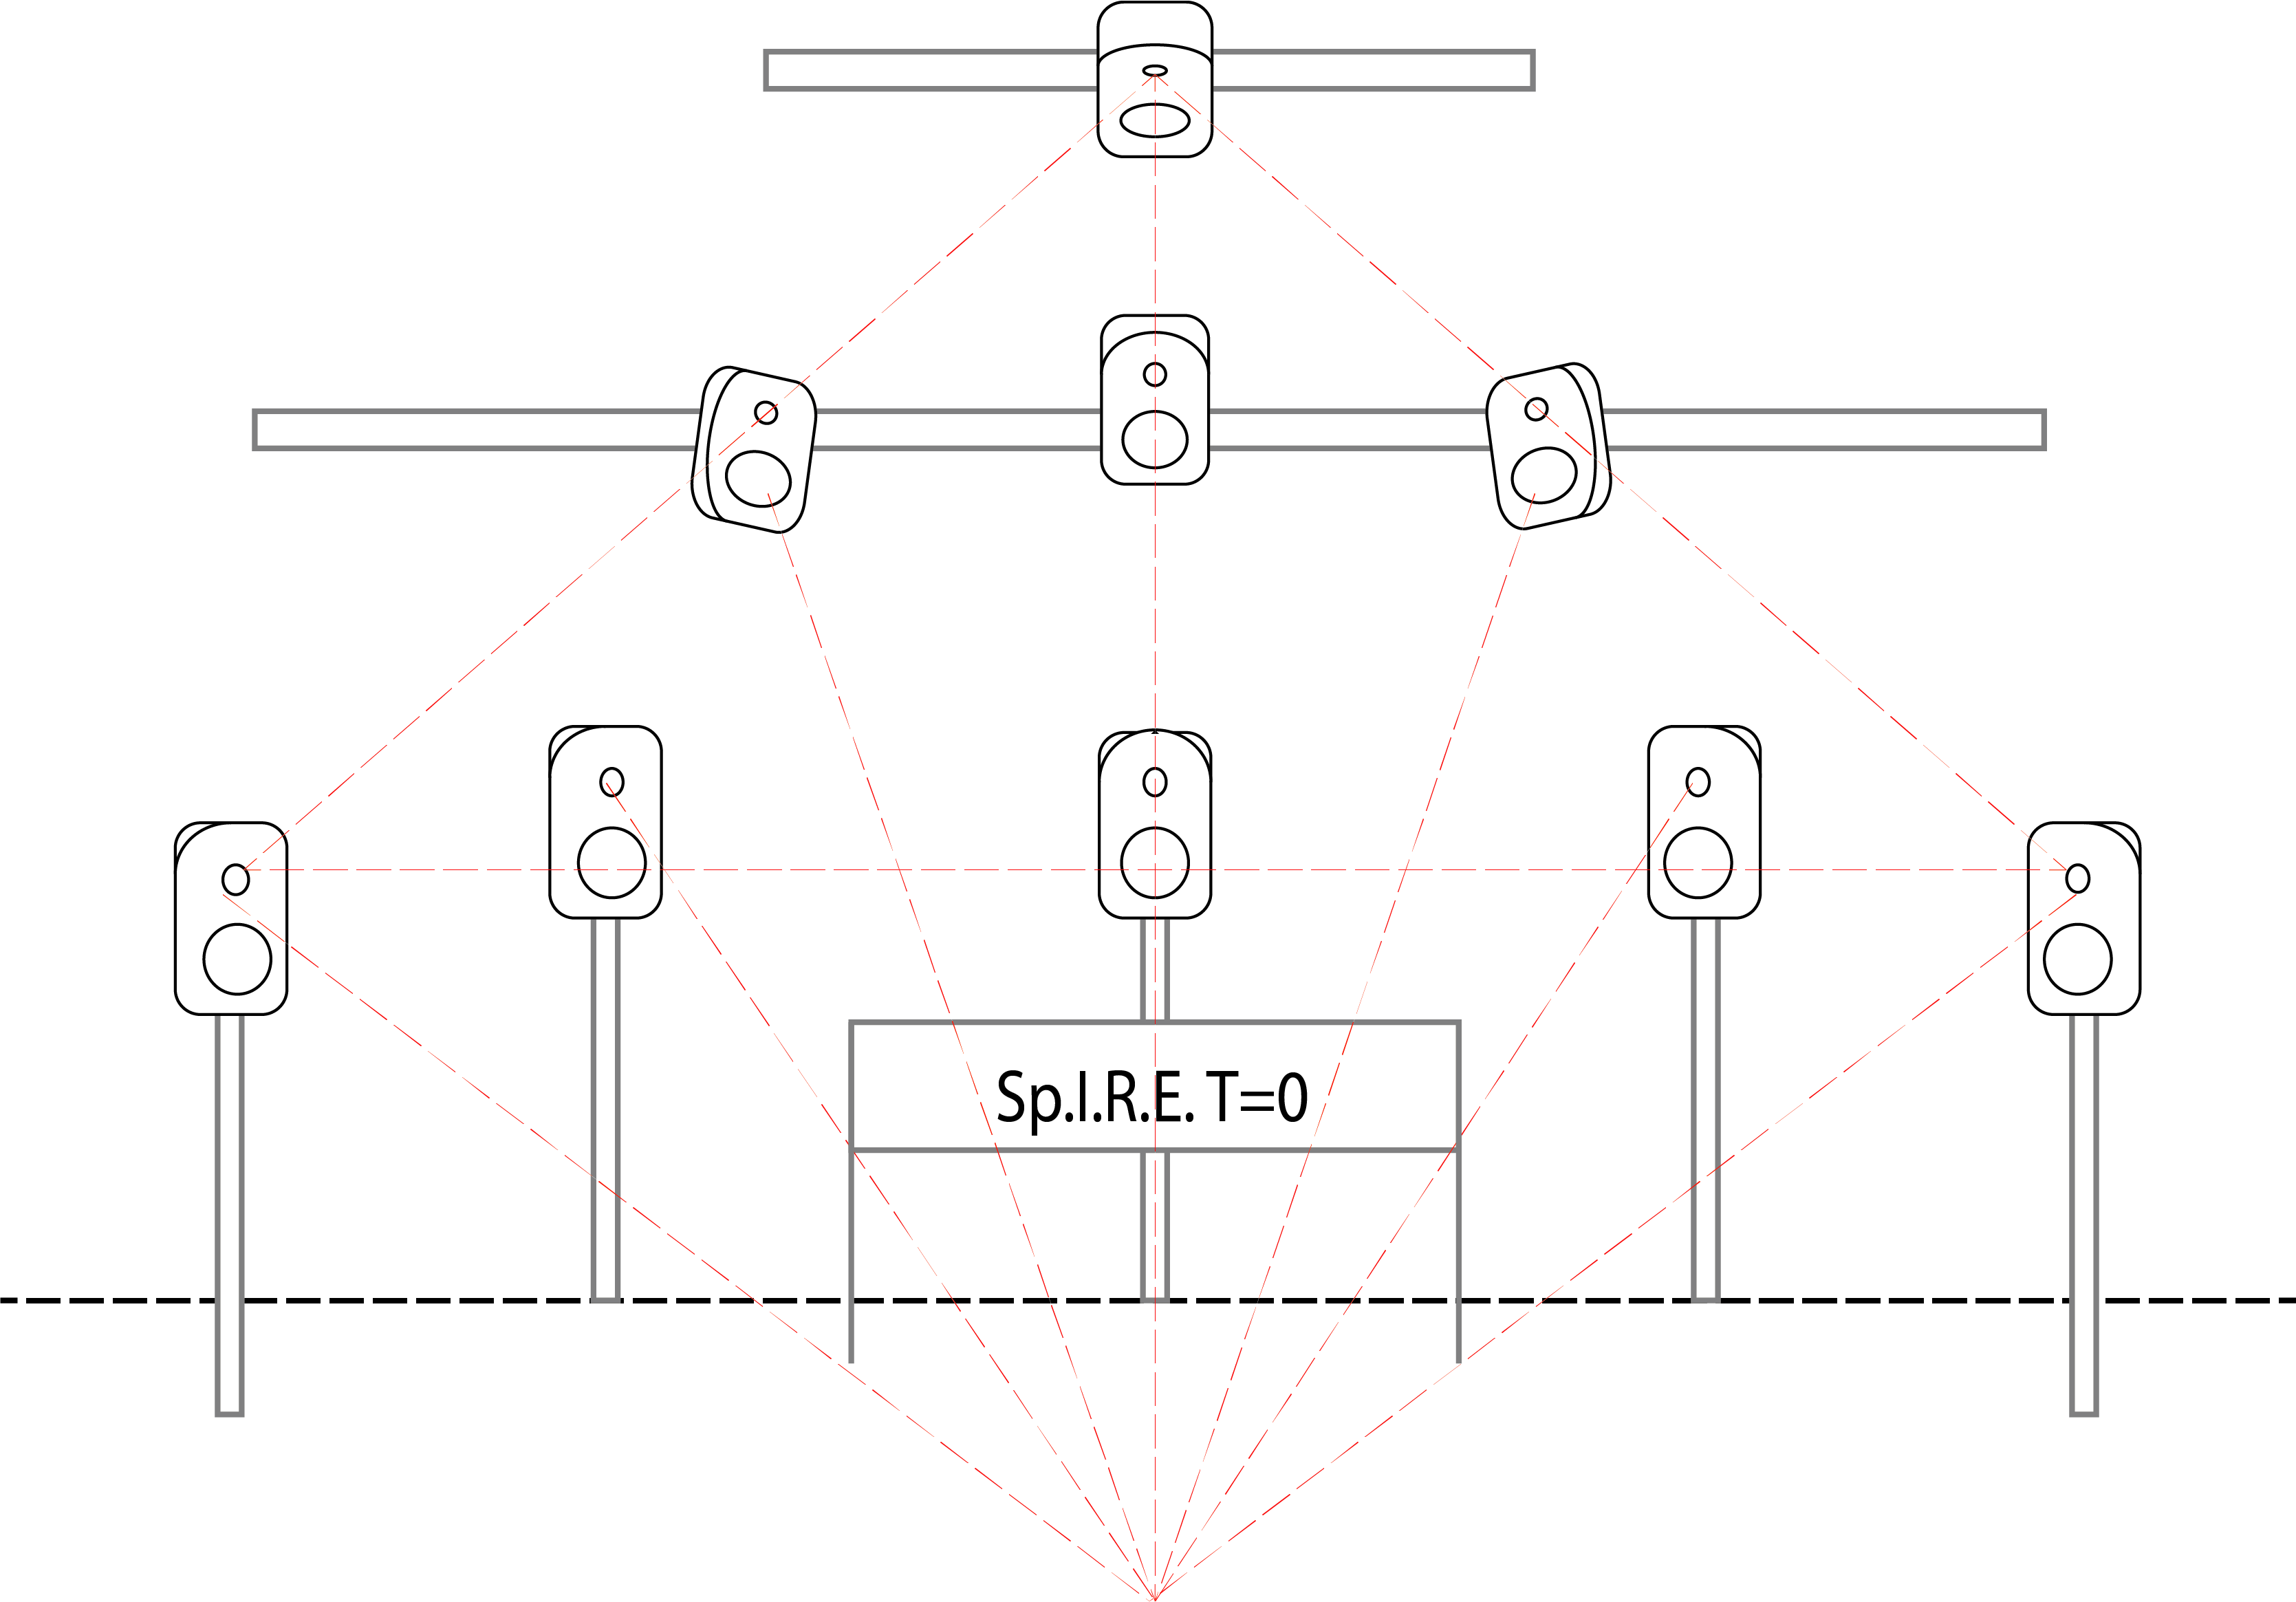
\includegraphics[width=.99\textwidth]{diffusione.png}
\caption{Diffusione a \textit{A Rosone} di Vitres de Son. \textit{Prospettiva}}
\label{default}
\end{center}
\end{figure}

\begin{itemize}
\item{La disposizione dei microfoni (figura 20) rende possibile un movimento spaziale del segnale. Sicuramente anche la scrittura ho tenuto conto di questo effetto, scrivendo gesti puntuali quando ritenevo strutturale uno spostamento della fonte sonora nello spazio.}
\item{La serie di filtri presente a valle, prima della diffusione, permette un movimento del suono verso l'alto, dato anche dall'utilizzo di diffusori sospesi al di sopra dello strumento}
\end{itemize}

L'amplificazione trasparente ed il filtraggio danno corporeità al suono e oltre a rendere possibile una spazializzazione realistica dello strumento, si da anche la possibilità alla stanza di risuonare su determinate frequenze dato il lungo decadimento dello Sp.I.R.E..
